\section{MapReduce}
现实中很多应用可以归结为这样一个模型,
MapReduce是一个编程模型,主要用于处理大的数据集,使用这个模型进行处理时,用户只需要提供两个函数:map和reduce,map函数处理输入的数据,产生中间的key/value键值对;reduce函数将具有相同key的中间结果归并,并产生最终结果。

使用MapReduce编程模型的一个最大优势在于,程序员不需要考虑底层的细节,由运行时系统管理并行,任务的分割,如何在集群环境中进行调度,容错,管理机器间的通信等等。程序员可以不用熟悉并行化,不了解分布式系统的情况下,能够最大化的利用分布式环境的资源

当处理的数据相当大的时候,考虑如何将输入的数据进行分割然后并行的处理,如何充分利用集群环境,如何容错成为关键的问题

MapReduce的最终目标是
hides the messy details of parallelization, fault-tolerance, data distribution and load balancing in a library.同时具有相当好的性能

MapReduce的实现方式有很多,主要看具体的机器和运行环境,Google的实现提供的是一种实现方式

\subsection{实现}
master通过ping来与worker进行检测,如果发现不通,就说明worker有问题
MapReduce目前无法处理master崩溃的情况,当master崩溃的话,就只能重启
{\color{red}那么如果要做容错?要如何改进}
\subsubsection{MapReduce的执行流程}
\begin{enumerate}
  \item user program首先会将输入数据分割成M份,然后在集群的机器中fork很多子程序。
  \item 多个程序中,有一个是master,其他都是worker,master会挑选一个空闲的worker,让它执行map任务或者reduce任务
  \item 执行map任务的worker,首先读取输入的内容,调用用户提供的map函数,产生中间键值对,将这些键值对存入到内存中,最后存入到local disk中
  \item map会周期性将内存中的内容写入到硬盘,然后将位置信息发送给master,然后master发送这些信息给reducer
  \item reduce接受到master发来的通知后,它会使用RPC(remote procedure calls)从map的disk中读取数据,然后reduce对读到的数据进行排序,这样相同key会在一起
  \item reduce调用用户提供的reduce函数,数据进行归并
  \item 当所有的map和reduce任务完成以后,master唤醒user program,mapreduce库结束,返回user code
\end{enumerate}

\subsubsection{Fault Tolerance}
1.worker failure
如果mapper出错,那么需要重新执行map task,因为不能从fail的机器中取出disk中的中间结果
如果reducer出错,那么不需要重新执行整个reduce task,因为reducer的结果存放于global file system
如果一个map task一开始执行于worker A,之后执行于worker B,那么所有的reducer就需要重新执行,因为reducer需要从B读取中间结果

2.master failure
目前的MapReduce中,因为只有一个master,还不能容错

How does MR cope with worker crashes?
  * Map worker crashes:
    master re-runs, spreads tasks over other GFS replicas of input.
      even if worker had finished, since still need intermediate data on disk.
    some Reduce workers may already have read failed worker's intermediate data.
      here we depend on functional and deterministic Map()!
    how does the master know the worker crashed? (pings)
    master need not re-run Map if Reduces have fetched all intermediate data
      though then a Reduce crash would have to wait for Maps to re-run
  * Reduce worker crashes before producing output.
    master re-starts its tasks on another worker.
  * Reduce worker crashes in the middle of writing its output.
    GFS has atomic rename that prevents output from being visible until complete.
    so it's safe for the master to re-run the Reduce tasks somewhere else.

Other failures/problems:
  * What if the master accidentally starts *two* Map() workers on same input?
    it will tell Reduce workers about only one of them.
  * What if two Reduce() workers for the same partition of intermediate data?
    they will both try to write the same output file on GFS!
    atomic GFS rename will cause the second to finish to win.
  * What if a single worker is very slow -- a "straggler"?
    perhaps due to flakey hardware.
    master starts a second copy of last few tasks.
  * What if a worker computes incorrect output, due to broken h/w or s/w?
    too bad! MR assumes "fail-stop" CPUs and software.
  * What if the master crashes?

\subsubsection{Locality}
网络带宽是非常稀缺的资源,因此应当尽量减少网络通信量,不仅如此,通过网络,也会存在一定的网络延迟。Google的MapReduce使用GFS作为文件的管理工具,输入文件存就放在集群中,MapReduce master会根据GFS提供的输入文件的copy的位置,并试图在存有输入文件的机器上启动任务,这样便可以避免网络的传输。(moving computation to data)

schedule a map task on a machine that contains a replica of the corresponding input data.
如果没有,那么会从最近的备份的机器中找,这样便具有好的局部性(Locality)

\subsubsection{Task Granularity}
map阶段的M pieces以及reduce阶段的R pieces,远远大于woker机器的数量,这样做的好处是,可以提高dynamic load balancing

\subsubsection{Backup Tasks}
map和reduce之间有一个barry,如果有一个map或者reduce特别慢,那么会增加这个MapReduce计算的total time
只有当map任务全部完成后,才会启动reduce任务,否则reduce无法获取全局的值
reduce的最终结果会写入到GFS

\subsection{Refinements}
几处可选的优化操作
\subsubsection{partition function}
reduce有R个,map产生的中间结果根据hash(key)\%R被发送给reduce,这样对于负载平衡有很大的好处

\subsubsection{combiner function}
将map产生的中间结果,进行局部的reduce操作,这样可以有小减少网路通信量,以及本地磁盘空间的使用
以word count为例,同一个key有1000个value,如果每个都是<key,1>那么需要存放1000次,需要通过网络发送1000次,如果进行局部的reduce那么就成为<key,1000>只要存放一个,然后发送一次

\subsection{总结}
MapReduce Model易于编程:it hides many painful details:
concurrency -- same result as sequential execution
starting s/w on servers
data movement
failures

This model scales well
map不需要等待其他的map也不需要共享数据,这样便可以并发的执行
reduce也一样

what will be the limiting factor in performance?
可以优化的地方在哪里?CPU? memory? disk? network?
They were limited by "network cross-section bandwidth",事实上,分布式环境下,最敏感的资源便是网络带宽,传输的量,以及网络延迟
但网络是外界的资源,很难去优化,我们能够做的是,尽量减少网络通信量
MapReduce做出的努力
\begin{itemize}
  \item Map input is read from local disks, not over network,尽量在存放input replication上启动map worker,这样便可以直接从local disk读取,而不是通过网络(moving computation to data)
  \item Map阶段的中间结果存放于local disk而不是GFS中,为什么?
  \item Intermediate data partitioned into files holding many keys,Big network transfers are more efficient
\end{itemize}

负载不均衡
How do they get good load balance?
理想的状态是每个server都能有相同的处理能力,然后或许相同的工作,最大的并发执行.
But time to process a split or partition isn't uniform.
Different sizes and contents, and different server hardware

解决的方案:many more splits than workers
Master hands out new splits to workers who finish previous tasks.
so no split is so big it dominates completion time.
这样的话,faster servers do more work than slower ones, finish about the same time

For what applications *doesn't* MapReduce work well?
  Not everything fits the map/shuffle/reduce pattern.
  Small data, since overheads are high. E.g. not web site back-end.
  Small updates to big data, e.g. add a few documents to a big index
  Unpredictable reads (neither Map nor Reduce can choose input)
  Multiple shuffles, e.g. page-rank (can use multiple MR but not very efficient)
  More flexible systems allow these, but more complex model.

因此MapReduce最大的优势是简单,但这种简单也限制了它对更多复杂应用程序的支持

\section{GFS}
GFS(Google File System)基于的一些假设:

1.GFS的服务器都是普通的商用计算机,并不那么可靠,集群出现结点故障是常态。因此必须时刻监控系统的结点状态,当结点失效时,必须能检测到,并恢复之。fault tolerance

2.系统存储适当数量的大文件。理想的负载是几百万个文件,文件一般都超过100MB,GB级别以上的文件是很常见的,必须进行有效管理。支持小文件,但不对其进行优化。

3.负载通常包含两种读:大型的流式读(顺序读)和小型的随机读。前者通常一次读数百KB以上,后者通常在随机位置读几个KB。

4.负载还包括很多连续的写操作,往文件追加数据(append)。文件很少会被修改,支持随机写操作,但不必进行优化。

5.系统必须实现良好定义的语义,用于多客户端并发写同一个文件。同步的开销必须保证最小。

6.高带宽比低延迟更重要,GFS的应用大多需要快速处理大量的数据,很少会严格要求单一操作的响应时间。

{\color{red}GFS期望的应用场景应该是大文件,连续读,不修改,高并发}

Google文件系统(Google File System,GFS)是构建在廉价的服务器之上的大型分布式系统。它将服务器故障视为正常现象,通过软件的方式自动容错,在保证系统可靠性和可用性的同时,大大减少了系统的成本。

GFS是Google云存储的基石,其它存储系统,如Google Bigtable,Google Megastore,Google Percolator均直接或者间接地构建在GFS之上。另外,Google大规模批处理系统MapReduce也需要利用GFS作为海量数据的输入输出。

\subsection{design}
\subsubsection{系统结构}
\begin{figure}[!ht]
    \centering
    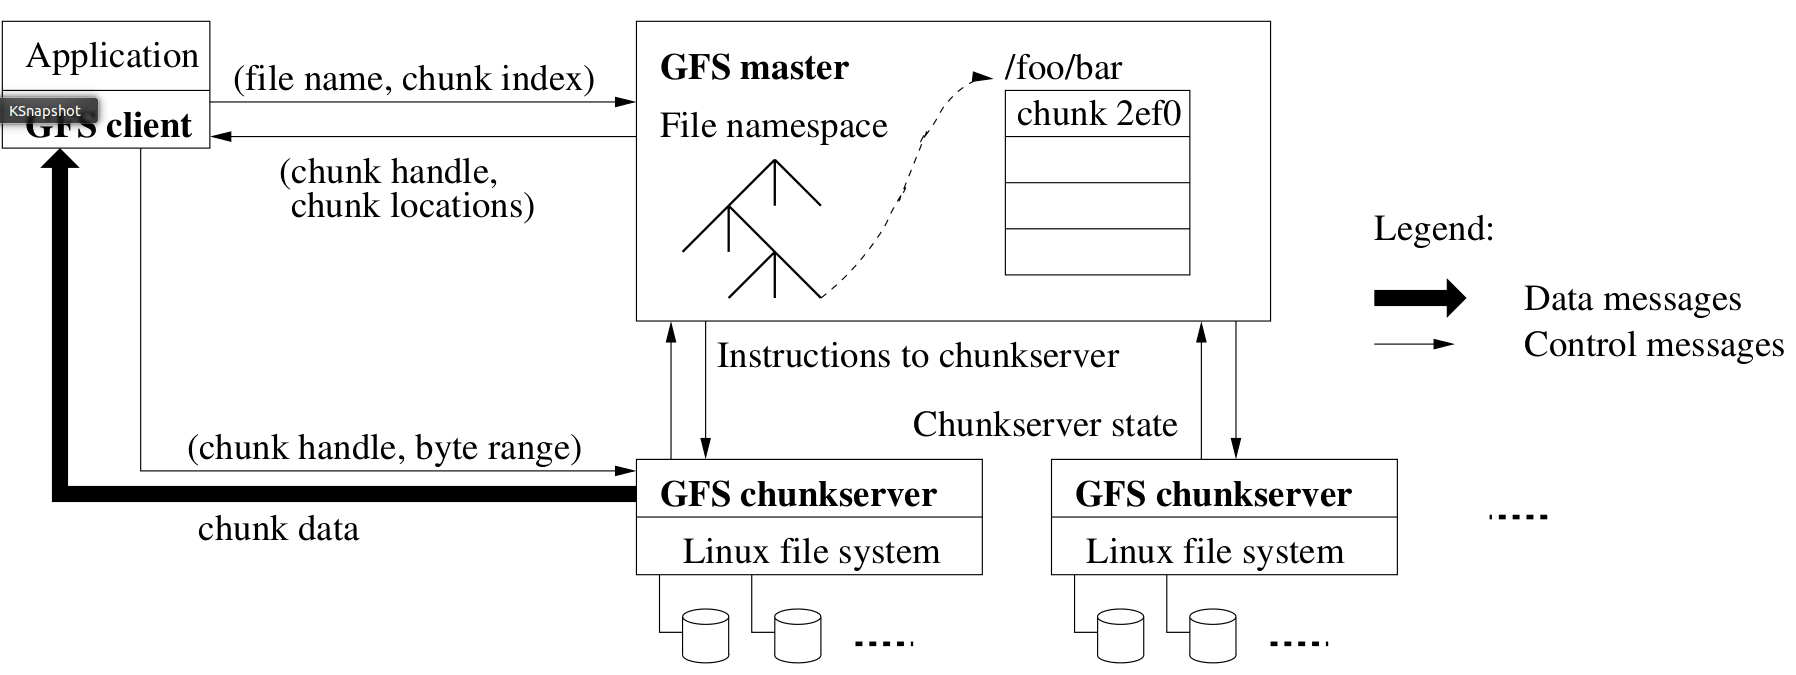
\includegraphics[height=7cm,width= 15cm]{img/gfs.png}
    \caption{gfs}
\label{gfs}
\end{figure}

GFS将整个系统的节点分为三种角色:GFS Master(总控服务器),GFS Chunkserver(数据块服务器,简称CS)以及GFS Client(客户端)。

chunkserver提供存储。GFS会将文件划分为定长数据块,
每个数据块都有一个全局唯一不可变的id(chunk\_handle),
数据块以普通Linux文件的形式存储在chunkserver上,
出于可靠性考虑,每个数据块会存储多个副本,分布在不同chunkserver,默认的情况为3个copy

GFS master就是GFS的元数据服务器,负责维护文件系统的元数据,包括命名空间、访问控制、文件-块映射、块地址等,以及控制系统级活动,如chunck lease的管理,垃圾回收、负载均衡等。master会周期性通过HeartBeat发送命令给chunkserver,或者收集它的状态信息

应用需要链接client的代码,然后client作为代理与master和chunkserver交互。master会定期与chunkserver交流(心跳),以获取chunkserver的状态并发送指令。

\subsubsection{single Master}
single Master的优势:简单(只需要读取全局数据有可以知道chunck的位置以及replication),可以避免出现脑裂的情况。
但这有可能造成一个问题:master的瓶颈,如果master的任务过重,会导致整个系统的性能被master限制,因此,尽量减少master的参与。另外一个很重要的问题便是“容错问题”,假设这个master崩溃了,怎么办?

为了避免master产生瓶颈,client不会直接通过master读写数据,而是先请求master,master告诉它与相应的chunckserver进行沟通,client会将这些信息存放在cache中一定的时间,这段时间里,将直接与相应的chunckserver进行沟通,无需master的参与

metadata
master中存放三种metadata: the file and chunk namespaces, the mapping from files to chunks, the locations of each chunk's replicas. 所有这些元数据都存放在master的内存中。
前两种are kept persistent.
master不会存储chunk locations persistent,而是动态的获取,通过HeartBeat messages.

{\color{red}日志的操作会更好一些}
\subsubsection{读GFS中的chunk}
GFS中的chunk的大小为64MB,“lazy space allocation”可以避免内部碎片浪费内存空间
1.选择一个大的chunk的advantage
\begin{itemize}
  \item reduce clients' need to interact with the master
  \item ?reduce network overhead by keeping a persistent TCP
  \item reduce the size of the metadata stored on the master 
\end{itemize}

2.disadvantage
\begin{itemize}
  \item 产生内部碎片,浪费空间,"lazy space allocation"可以避免
  \item The chunkservers storing those chunks may become hot spots if many clients are accessing the same file
\end{itemize}


Client读GFS中的chunk

1.应用指定读取某个文件的某段数据,因为数据块是定长的,
client可以计算出这段数据跨越了几个数据块,
client将文件名和需要的数据块索引发送给master;

2.master根据文件名查找命名空间和文件-块映射表,得到需要的数据块副本所在的地址,
将数据块的id和其所有副本的地址反馈给client;

3.client选择一个副本,联系chunkserver索取需要的数据;

4.chunkserver返回数据给client。

\subsubsection{consistency Model}
\subsubsection{一致性}
GFS必须将对数据块的修改同步到每一个副本。考虑一下多个应用同时修改同一数据块的情况,
我们必须为修改操作定义统一的时序,不然多个副本会出现不一致的情况,
那么定义时序由谁做呢?还记得前面提到的元数据缓存么,
为了减少master的负担,client在获得副本位置后就不再和master交互,
所以必然需要选出一个master代理来完成这个任务。
事实上GFS采用了租约(lease)的机制,master会将租约授权给某个副本,称为primary,
由这个primary来确定数据修改的顺序,其它副本照做就是。

Client写
\begin{figure}[!ht]
    \centering
    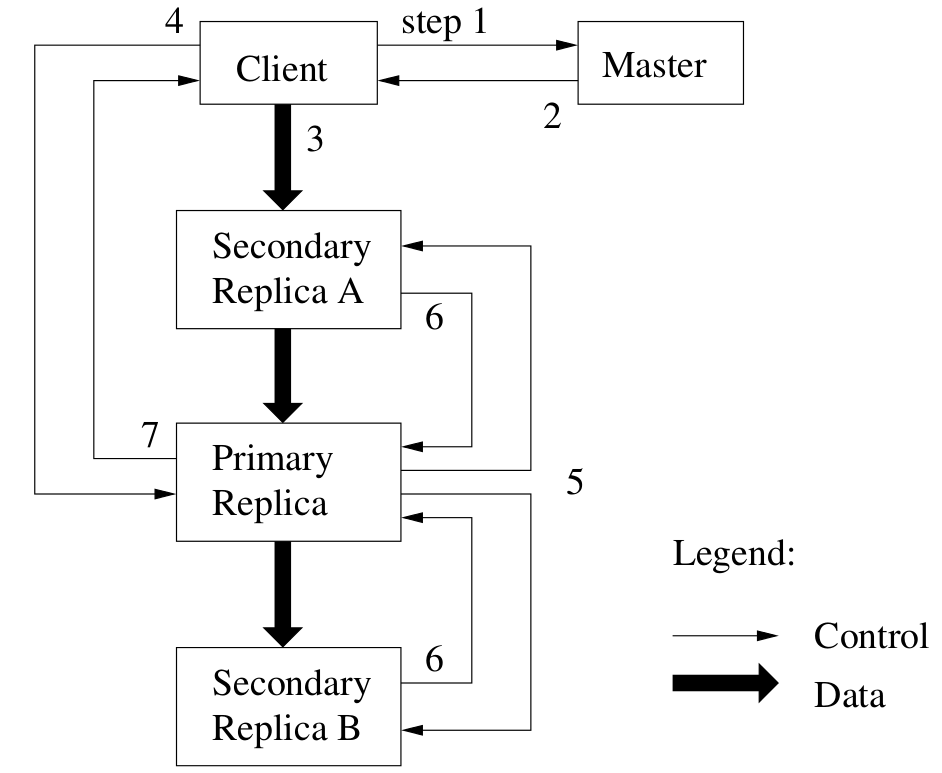
\includegraphics[height=8cm,width= 9cm]{img/gfs_write.png}
    \caption{gfs write}
\label{gfs_write}
\end{figure}

1.client需要更新一个数据块,询问master哪个chunkserver拥有该数据块的lease(谁是primary)以及其他replicas(副本)的位置;

2.master将持有lease的primary和其它副本的位置告知client,client缓存之;只有当primary不可达或者不再持有lease的时候,client才会向master发出请求。

3.client向所有副本传输数据,这里副本没有先后顺序,根据网络拓扑情况找出最短路径,数据从client出发沿着路径流向各个chunkserver,这个过程采用流水线(网络和存储并行)。chunkserver将数据放到LRU缓存;

4.一旦所有的副本都确定接受数据,client向primary发送写请求,
primary为所有的写操作分配连续的序列号表示先后顺序,
并且按照顺序执行数据更新;

5.primary将写请求发送给其它副本,每个副本都按照primary确定的顺序执行更新;

6.其它副本向primary汇报操作情况;

7.primary应答client操作情况,任何副本错误都导致此次请求失败,
并且此时副本处于不一致状态(写操作完成情况不一样)。client会尝试几次3到7的步骤,实在不行就只能重头来过了。

\subsection{consistency}
Weak consistency: read() may return stale data ---not the result of the most recent write
Strong consistency read() always returns the data from the most recent write()
nice for applications writers, but bad for performance


理想的consistency model是:A replicated files behaves like as a non-replicated file system
多个clients在读取的时候,仿佛在操作同一个机器的一个disk

导致不一致的操作:
concurrency(并发),Machine failures, Network partitions

为了获取更好的性能和设计的简单,GFS 并没有使用最理想的一致性模型

store 64MB chunks (an ordinary Linux file for each chunk)
    each chunk replicated on three servers
    Q: why 3x replication?
    Q: Besides availability of data, what does 3x replication give us?
       load balancing for reads to hot files(因为有三份copy,读的时候,具有较高的并发和好的load balance)
       affinity
    Q: why not just store one copy of each file on a RAID'd disk?
       RAID isn't commodity
       Want fault-tolerance for whole machine; not just storage device
    Q: why are the chunks so big?
    
\subsection{fault tolerance}
  Single master
    Clients always talk to master
    Master orders all operations
  Stores limited information persistently
    name spaces (directories)
    file-to-chunk mappings
  Log changes to these two in a log
    log is replicated on several backups
    clients operations that modify state return *after* recording changes in *logs*
    logs play a central role in many systems we will read about
    logs play a central role in labs
  Limiting the size of the log
    Make a checkpoint of the master state
    Remove all operations from log from before checkpoint
    Checkpoint is replicated to backups
  Recovery
    replay log starting from last checkpoint
    chunk location information is recreated by asking chunk servers
  Master is single point of failure
    recovery is fast, because master state is small
      so maybe unavailable for short time
    shadow masters
      lag behind master
        they replay from the log that is replicated
      can server read-only operations, but may return stale data
    if master cannot recovery, master is started somewhere else
    must be done with great care to avoid two masters
  We will see schemes with stronger guarantees, but more complex
    see next few lectures

Chunk fault tolerance
  Master grants a chunk lease to one of the replicas
    That replica is the primary chunk server
  Primary determines orders operations
  Clients pushes data to replicas
    Replicas form a chain
    Chain respects network topology
    Allows fast replication
  Client sends write request to primary
    Primary assigns sequence number
    Primary applies change locally
    Primary forwards request to replicates
    Primary responds to client after receiving acks from all replicas
  If one replica doesn't respond, client retries
  Master replicates chunks if number replicas drop below some number
  Master rebalances replicas
  
  Consistency model
  Strong consistency for directory operations
    Master performs changes to metadata atomically
    Directory operations follow the "ideal"
    But, when master is off-line, only shadow masters
      Read-only operations only, which may return stale data
  Weak consistency for chunk operations
    A failed mutation leaves chunks inconsistent
      The primary chunk server updated chunk
      But then failed and the replicas are out of date
    A client may read an not-up-to-date chunk
    When client refreshes lease it will learn about new version 
  Authors claims weak consistency is not a big problems for apps    
    Most file updates are append-only updates
      Application can use UID in append records to detect duplicates
      Application may just read less data (but not stale data)
    Application can use temporary files and atomic rename
\subsection{GFS与HDFS以及os的FS对比}
